\documentclass{article}
\usepackage{fontspec}
\pagestyle{empty}
\usepackage{geometry}
\geometry{paperwidth=50mm, paperheight=40mm, left=2mm, top=0mm, right=2mm, bottom=0mm}
\parindent=0pt
\usepackage{color}
\usepackage{xcolor}
\usepackage{tikz}
\usetikzlibrary{calc} 

\begin{document}
\centering
\vspace*{\fill} \vspace*{-5ex}
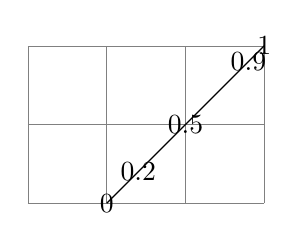
\begin{tikzpicture}
\draw [help lines] (0,0) grid (3,2);
\draw (1,0) -- (3,2);
\foreach \i in {0,0.2,0.5,0.9,1}
\node at ($(1,0)!\i!(3,2)$) {\i};
\end{tikzpicture}

\vspace*{\fill} 
\end{document}